\documentclass[a4paper]{article}
\usepackage[warn]{mathtext}
\usepackage[utf8]{inputenc}
\usepackage[T2A]{fontenc}
\usepackage[english,russian]{babel}
\usepackage{indentfirst}
\usepackage{misccorr}
\usepackage{subcaption}
\captionsetup{compatibility=false}
\usepackage{geometry}
\geometry{verbose,a4paper,tmargin=2cm,bmargin=2cm,lmargin=1.5cm,rmargin=1.5cm}
\usepackage{graphicx}
\usepackage{wrapfig}
\usepackage{amsmath}
\usepackage{fancyhdr}
\usepackage{floatflt}
\usepackage{float}
\usepackage{amssymb}
\usepackage{color}
\usepackage{lscape}
\usepackage{hvfloat}
\usepackage{amsfonts}
\usepackage{euscript}
\usepackage{newunicodechar}
\usepackage{listings}



\usepackage{xcolor}
\usepackage{hyperref}
% Цвета для гиперссылок
\definecolor{linkcolor}{HTML}{000000} % цвет ссылок
\definecolor{urlcolor}{HTML}{000070} % цвет гиперссылок

\definecolor{dkgreen}{rgb}{0,0.6,0}
\definecolor{gray}{rgb}{0.5,0.5,0.5}
\definecolor{mauve}{rgb}{0.58,0,0.82}

\hypersetup{pdfstartview=FitH,  linkcolor=linkcolor,urlcolor=urlcolor, colorlinks=true}

\lstset{
  language=Java,
  aboveskip=3mm,
  belowskip=3mm,
  showstringspaces=false,
  columns=flexible,
  basicstyle={\small\ttfamily},
  numbers=none,
  numberstyle=\tiny\color{gray},
  keywordstyle=\color{blue},
  commentstyle=\color{dkgreen},
  stringstyle=\color{mauve},
  breaklines=false,
  breakatwhitespace=true,
  tabsize=3
}

\begin{document}


\begin{titlepage}
	\centering
    
	\vspace{10cm}
	{\scshape\LARGE  Отчет по практическому заданию №1 \par}
	\vspace{1cm}
	{\huge\bfseries  Объектно-ориентированное программирование в Java\par}
	\vspace{1cm}
	\vfill
\begin{flushright}
	{\large Выполнила:}\par
	\vspace{0.3cm}
    {\LARGE Юлия Прохорова}
Zhbxtr
\end{flushright}
	
	\vfill

% Bottom of the page
	2021 г.
\end{titlepage}

\newpage

\pagestyle{fancy} 
\fancyhead[R]{ООП в Java}
\fancyhead[L]{Юлия Прохорова}
\fancyhead[C]{}
\fancyfoot{}
\fancyfoot[C]{ \noindent\rule{\textwidth}{0.4pt} \thepage }

\tableofcontents

\newpage

\newcommand{\RNumb}[1]{\uppercase\expandafter{\romannumeral #1\relax}}


\section{\href{https://github.com/julproh/5_sem/tree/main/NetCracker/Java_Basics_and_OOP/first_task/equations}{Решение квадратных уравнений}}

\begin{enumerate}
    \item Реализация программы:
    \begin{lstlisting}
    package equations;

    import java.util.Scanner;

    public class SolvingEquation{ 
        public static void main (String[] args) {
            double[] coefficient = new double[3]; 
            Scanner in = new Scanner(System.in);
            for (int i = 0; i < coefficient.length; i++) {
                coefficient[i] = in.nextDouble(); 
            }
            in.close();
            if (coefficient[0] == 0 && coefficient[1] != 0  ) { 
                System.out.println("Solution: " + -coefficient[2]/coefficient[1] );
            } 
            else if (coefficient[0] == 0 && coefficient[1] == 0 && coefficient[2]!=0) {
                System.out.println("The equation has no solution");
            }
            else if (coefficient[0] == 0 && coefficient[1] == 0 && coefficient[2]==0) {
                System.out.println("The equation has infinitely many solutions");
            }
            else {
                Equations equation_ = new Equations(coefficient[0], coefficient[1], coefficient[2]);
                equation_.answer(equation_.discriminant_.discriminant(equation_.a, equation_.b, equation_.c));
            }
        }
    }

    class Equations {
        public double a, b, c; // a*x*x+b*x+c=0 - equation
        Discriminant discriminant_ = new Discriminant();

        Equations(double a, double b, double c) {
            this.a = a;
            this.b = b;
            this.c = c;
        }

        class Discriminant {
            public double discriminant (double a, double b, double c) {
                double q_discriminant = b*b - 4*a*c;
                double _discriminant;
                if (q_discriminant >= 0) {
                    _discriminant =  Math.sqrt(q_discriminant);
                } 
                else {
                    _discriminant = -1;
                }
                return _discriminant;
            };
        }
    
        public void answer (double _discriminant) {

            if (_discriminant < 0) {
                System.out.println("No Real Solutions");
            }
            else if (_discriminant == 0) {
                System.out.println("Solution: " + -this.b/2/this.a);
            }
            else {
                System.out.println("Solution: " + (-this.b+_discriminant)/2/this.a);
                System.out.println("Solution: " + (-this.b-_discriminant)/2/this.a);
            }
        }
    }

\end{lstlisting}

    \item Результаты тестов:
        
        \begin{figure}[h!]
            \begin{center}
                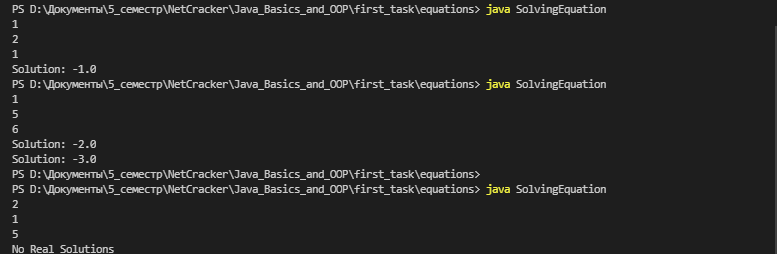
\includegraphics[scale = 0.6]{test_t1.png}
                \label{p2} %% метка рисунка для ссылки на него
            \end{center}
        \end{figure}
    
    \item Структура class файлов:
    \\
    Весь исходный код сначала компилируется в байт-код с помощью компилятора javac, входящего в состав Java Development Kit. 
    Байт-код сохраняется в бинарный файл в специальный class-файл. Затем эти class-файлы загружаются в память загрузчиком классов (ClassLoader).
    Каждый файл с расширением .java компилируется как минимум в один файл .class. Для каждого класса создается по одному .class файлу. Это также относится к интерфейсам и вложенным классам.
    Состав class-файла:
    \begin{enumerate}
        \item Cигнатура - первые 4 байта, идентифцирующие его.
        \item Версия файла.
        \item Пул констант - строковые константы, имена классов, интерфейсов, полей, методов и тд. 
        \item Флаги доступа.
        \item This class.
        \item Super class.
        \item Количество интерфейсов, реализованных классом.
        \item Количество полей в классе или интерфейсе.Описание полей.
        \item Количество методов и описание методов.
        \item Количество атрибутов. Атрибутыю
    \end{enumerate}
    
    \item Использование вложенного класса:
    \\
    Вложенный класс создается для того, чтобы обслуживать окружающий его класс. 
    Внутренний класс ведет себя как обычный класс за тем исключением, что его объекты могут быть созданы только внутри внешнего класса.

    Внутренний класс имеет доступ ко всем полям внешнего класса. Аналогично внешний класс имеет доступ ко всем членам внутреннего класса, в том числе к полям и методам с модификатором private.

    \item Чтобы перейти к реализации программы на Github, нажмите на название задачи в самом начале ее описания.
    
    

    
\end{enumerate}

\section{\href{https://github.com/julproh/5_sem/tree/main/NetCracker/Java_Basics_and_OOP/first_task/bones}{Игра в кости}} 

    \begin{enumerate}

        \item Реализация программы:
        \begin{lstlisting}
package bones;

import java.util.Random;
import java.util.Scanner;


public class Bones {

    public static void main (String[] args) {

        int n, k;

        System.out.println("Print the number of the players with the computer");

        Scanner in = new Scanner(System.in);
        n = in.nextInt();

        System.out.println("Print the number of the bones");
        k = in.nextInt();
        in.close();
    
        int[][] players = new int[2][n];
        for  (int i = 0; i < n; i++) {
            players[0][i] = i+1;
            players[1][i] = 0;
        }
        int[] current = new int [n];

        int winner = 0;
        int max = 0;
        int flag = 0;

        final Random random = new Random();

        while (flag == 0) {
            for (int i = 0; i < n; i++){
                for (int j = 0; j < k; j++) {
                    
                    current[i] += random.nextInt(5) + 1; 
                }
                if ( current[i] > max) {
                    max = current[i];
                    winner = i;
                }
            };
            players[1][winner]++;
            if (players[1][winner]==7){
                flag = 1;
            } 
            else {
                int number = players[1][winner];
                for(int i = winner; i > 0; i--) {
                    players[0][i] = players[0][i-1];
                    players[1][i] = players[1][i-1];
                }
                players[0][0] = winner+1;
                players[1][0] = number;
                for (int i=0; i < n; i++) {
                    current[i] = 0;
                }

            }
        };

        System.out.println("The winner is " + players[0][0] + " player");

    };
}
        \end{lstlisting}
    
        \item Результаты тестов:
        
        \begin{figure}[h!]
            \begin{center}
                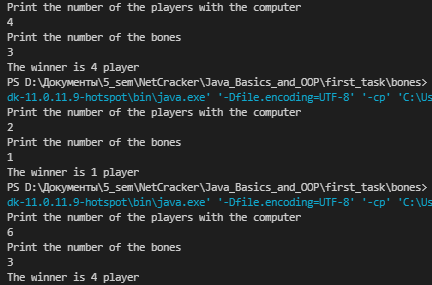
\includegraphics[scale = 0.8]{test_t2.png}
                \label{p2} %% метка рисунка для ссылки на него
            \end{center}
        \end{figure}

        \item Чтобы перейти к реализации программы на Github, нажмите на название задачи в самом начале ее описания.
    
    \end{enumerate}

\section{\href{https://github.com/julproh/5_sem/tree/main/NetCracker/Java_Basics_and_OOP/first_task/address}{Адрес человека}}

    \begin{enumerate}
   
        \item Реализация программы:
        
        \begin{lstlisting}
            package address;

            import java.util.Calendar;
            import java.util.GregorianCalendar;
            import java.util.Date;
            
            
            class Person {
                String name;
                String surname;
                Calendar dateOfBirth;
                Address address;
            
                Person(String _name, String _surname, Calendar _dateOfBirth) {
                    name = _name;
                    surname = _surname;
                    dateOfBirth = _dateOfBirth;
                };
            
                class Address {
                    int flat;
                    int house;
                    String street;
                    String city;
                    String country;
                    
                    Address () {};
            
                    Address(int _flat, int _house, String _street, String _city,  String _country) {
                        flat = _flat;
                        house = _house;
                        street = _street;
                        city = _city;
                        country = _country; 
                    };
            
                    void printAddress () {
                        System.out.print(country + " " + city + " " + street + " " + house + " " + flat);
                    }
                }
            
                void printInformation () {
                    System.out.println("Name: " + this.name);
                    System.out.println("Surname: " + this.surname);
                    Date date = dateOfBirth.getTime();
                    System.out.println("Date of birth: " + date);
                    System.out.print("Address: ");
                    this.address.printAddress();
            
                }
            }
            
            public class OperationsWithPeople {
                
                static void findBySurname(String _surname, Person[] _people) {
                    int k = 0;
                    for (int i = 0; i < _people.length; i++) {
                        if (_people[i].surname == _surname) {
                            k++;
                            _people[i].printInformation();
                            System.out.println("\n _____________");
                        } 
                        if (k == 0) {
                            System.out.println("There is no person with such surname");
                        }
                    }
                }
            
                static void findByFlat (int _flat, Person[] _people) {
                    int k = 0;
                    for (int i = 0; i < _people.length; i++) {
                        if (_people[i].address.flat == _flat) {
                            k++;
                            _people[i].printInformation();
                            System.out.println("\n _____________");
                        } 
                        if (k == 0) {
                            System.out.println("There is no person with such flat");
                        }
                    }
                }
                static void findByHouse (int _house, Person[] _people) {
                    int k = 0;
                    for (int i = 0; i < _people.length; i++) {
                        if (_people[i].address.house == _house) {
                            k++;
                            _people[i].printInformation();
                            System.out.println("\n _____________");
                        } 
                        if (k == 0) {
                            System.out.println("There is no person with such house");
                        }
                    }
                }
                
                static void findByStreet (String _street, Person[] _people) {
                    int k = 0;
                    for (int i = 0; i < _people.length; i++) {
                        if (_people[i].address.street == _street) {
                            k++;
                            _people[i].printInformation();
                            System.out.println("\n _____________");
                        } 
                        if (k == 0) {
                            System.out.println("There is no person with such street");
                        }
                    }
                }
            
                static void findByCity (String _city, Person[] _people) {
                    int k = 0;
                    for (int i = 0; i < _people.length; i++) {
                        if (_people[i].address.city == _city) {
                            k++;
                            _people[i].printInformation();
                            System.out.println("\n _____________");
                        } 
                        if (k == 0) {
                            System.out.println("There is no person with such city");
                        }
                    }
                }
            
                static void findByCountry (String _country, Person[] _people) {
                    int k = 0;
                    for (int i = 0; i < _people.length; i++) {
                        if (_people[i].address.country == _country) {
                            k++;
                            _people[i].printInformation();
                            System.out.println("\n _____________");
                        } 
                    }
                    if (k == 0) {
                        System.out.println("There is no person with such country");
                    }
                }
            
                static void findTheMostOld (Person[] _people) {
                    int k = 0;
                    for (int i = 1; i < _people.length; i++) {
                        Date datek = _people[k].dateOfBirth.getTime();
                        Date datei = _people[i].dateOfBirth.getTime();
                        if (datek.getTime() > datei.getTime()) {
                            k = i;
                        }
                    }
                    _people[k].printInformation();
                    System.out.println("\n _____________");
                }
            
                static void findTheYoungest (Person[] _people) {
                    int k = 0;
                    for (int i = 1; i < _people.length; i++) {
                        Date datek = _people[k].dateOfBirth.getTime();
                        Date datei = _people[i].dateOfBirth.getTime();
                        if (datek.getTime() < datei.getTime()) {
                            k = i;
                        }
                    }
                    _people[k].printInformation();
                    System.out.println("\n _____________");
                }
            
                static void findBetween (Calendar _date1, Calendar _date2, Person[] _people) {
                        Date date1 = _date1.getTime();
                        Date date2 = _date2.getTime();
                    for (int i = 1; i < _people.length; i++) {
                        Date date = _people[i].dateOfBirth.getTime();
                        if ((date.getTime() >= date1.getTime() && date.getTime() <= date2.getTime()) 
                        || (date.getTime() <= date1.getTime() && date.getTime() >= date2.getTime())  ) {
                            _people[i].printInformation();
                            System.out.println("\n _____________");
                        }
                    }
                }
            
                public static void main (String[] args) {
                    Person[] people = new Person[4];
                    
                    people[0] = new Person("Ivan", "Petrov", new GregorianCalendar(2001, 01, 01) );
                    people[0].address = people[0].new Address(1,1,"First", "Ivanovo", "Russia");
                    people[1] = new Person("Ivan", "Ivanov", new GregorianCalendar(2001, 02, 01));
                    people[1].address = people[1].new Address(1, 2, "Second", "Moscow", "Russia");
                    people[2] = new  Person("Andrew", "Petrov", new GregorianCalendar(1991, 8, 11));
                    people[2].address = people[2].new Address(1, 1, "First", "Dolgoprudny", "Russia" );
                    people[3] = new Person("Olga", "Sowa", new GregorianCalendar(2010, 8, 05));
                    people[3].address = people[3].new Address(10, 5, "Pobeda", "Kiev", "Ukraine");
            
                    System.out.println("Found by city:");
                    findByCity("Ivanovo", people);
                    System.out.print("\n");
                    System.out.println("Find by country:");
                    findByCountry("America", people);
                    System.out.print("\n");
                    System.out.println("Find by flat:");
                    findByFlat(1, people);
                    System.out.print("\n");
                    System.out.println("Find by house:");
                    findByHouse(5, people);
                    System.out.print("\n");
                    System.out.println("Find by street:");
                    findByStreet("Pobeda", people);
                    System.out.print("\n");
                    System.out.println("Find by surname:");
                    findBySurname("Ivanov", people);
                    System.out.print("\n");
                    System.out.println("The oldest:");
                    findTheMostOld(people);
                    System.out.print("\n");
                    System.out.println("The youngest:");
                    findTheYoungest(people);
                    System.out.print("\n");
                    System.out.println("People between dates:");
                    findBetween(new GregorianCalendar(2000, 8, 9), new GregorianCalendar(2005, 6, 9), people);
                    System.out.print("\n");
            
                };
            
            
            
            }
        \end{lstlisting}
        \item Результаты тестов:
        
        \begin{figure}[h!]
            \begin{center}
                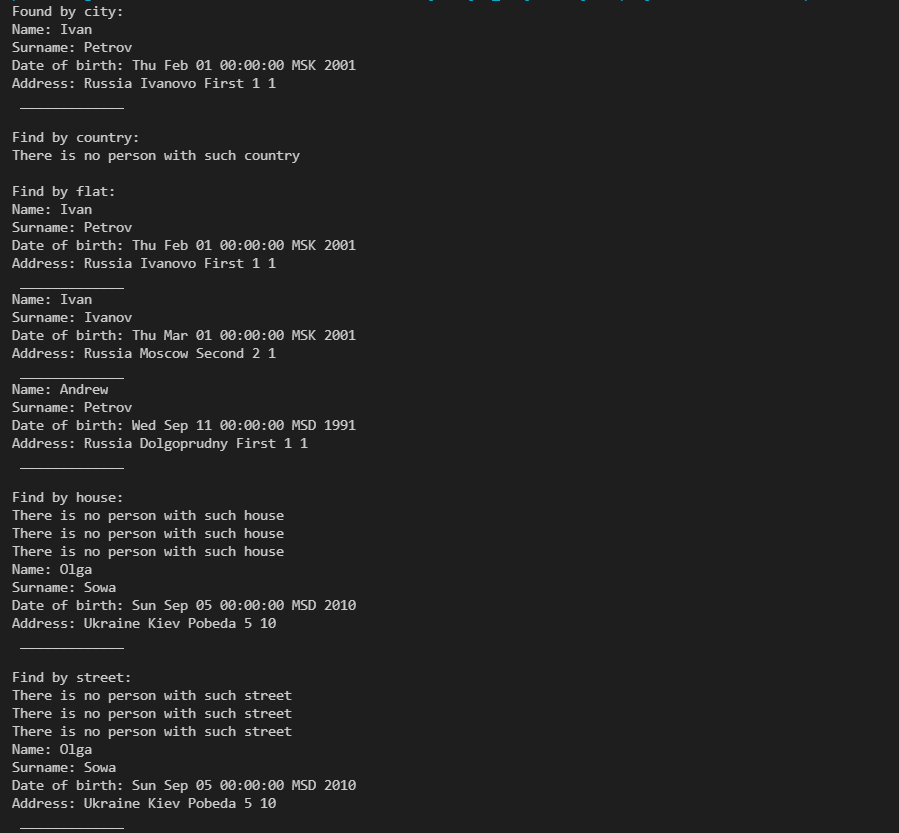
\includegraphics[scale = 0.6]{test_t3_p1.png}
                \label{p2} %% метка рисунка для ссылки на него
            \end{center}
        \end{figure}

        \begin{figure}[H]
            \begin{center}
                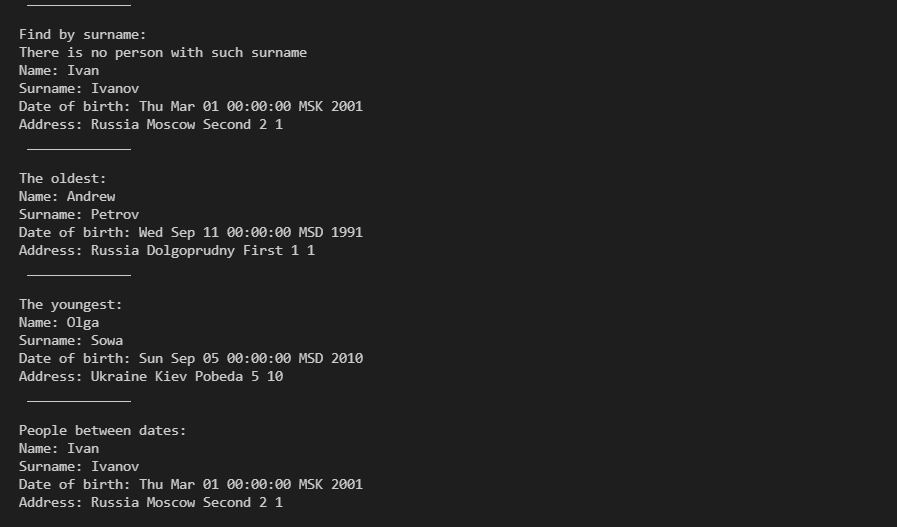
\includegraphics[scale = 0.6]{test_t3_p2.png}
                \label{p2} %% метка рисунка для ссылки на него
            \end{center}
        \end{figure}
        \item Чтобы перейти к реализации программы на Github, нажмите на название задачи в самом начале ее описания.
    
    \end{enumerate}

\end{document}